\section*{Задача 2.3}
Используя метод Ньютона найти все корни алгебраического уравнения  $P_m(x) = 0$ с точностью $\varepsilon = 10^{-8}$.
\[P_m(x) = x^5 - 5.1 x^4 + 9.6 x^3 + 9.8 x^2 - 8.8x - 5.\]

\subsection*{Решение}
Графически найдем отрезки локализации для вещественных корней, за начальные приближения возьмем середины отрезков.

\includegraphics[width=\textwidth]{231.eps}

Результат применения метода Ньютона:
\begin{verbatim}
Выполнено 4 итераций. x = -0.89479384
Выполнено 4 итераций. x = -0.46653499
Выполнено 4 итераций. x = 0.93485047
\end{verbatim}

Для поиска комплексных корней уравнения построим график на комплексной плоскости, где большим значениям функции соответствуют более светлые цвета и наоборот.

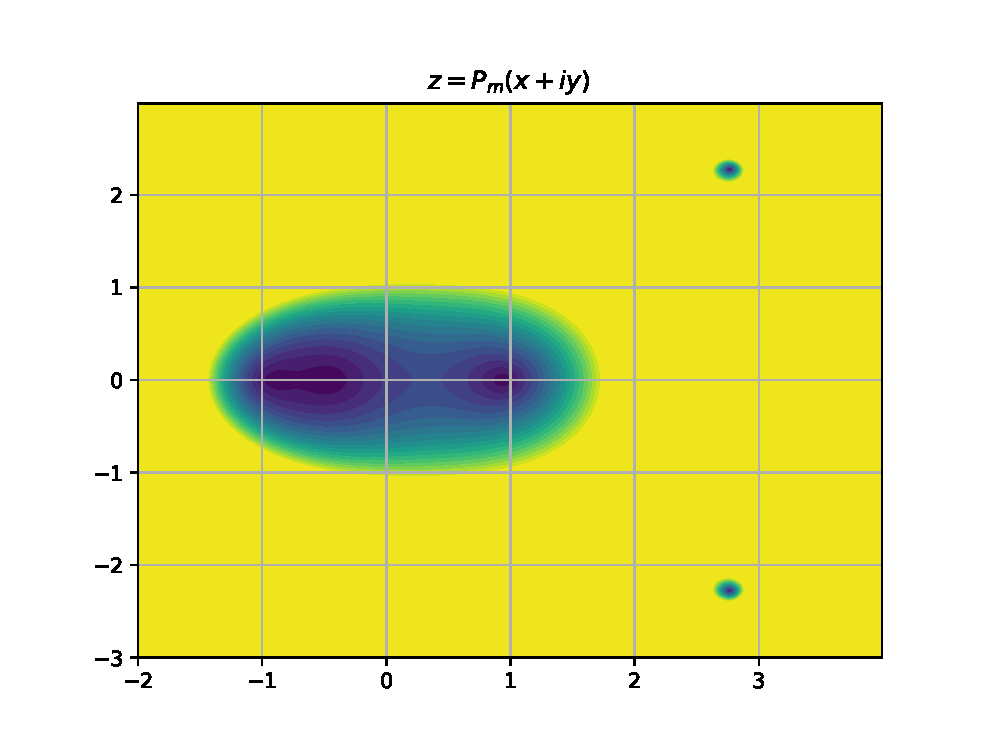
\includegraphics[width=\textwidth]{232.eps}

На графике, кроме трех вещественных корней, видны также два комплексных корня в окрестностях точек $2.8+2.5i$ и $2.8-2.5i$. Запустим из них метод Ньютона, чтобы узнать точные значения этих корней:
\begin{verbatim}
Выполнено 5 итераций. x = 2.76323918-2.27521843j
Выполнено 5 итераций. x = 2.76323918+2.27521843j
\end{verbatim}

Таким образом уравнение $P_m(x) = 0$ имеет пять алгебраических корней:
\begin{gather*}x_1 = -0.89479384,\\
    x_2 = -0.46653499,\\
    x_3 = 0.93485047,\\
    x_4 = 2.76323918-2.27521843i,\\
    x_5 = 2.76323918+2.27521843i.
\end{gather*}
